%
% vektorprodukt.tex
%
% (c) 2018 Prof Dr Andreas Müller, Hochschule Rapperswil
%

\section{Vektorprodukt}
Das orientierte Volumn in drei Dimensionen ermöglicht die Konstruktion 
des Vektorproduktes.
Mit ihm wird die Aufgabe, einen Vektor senkrecht auf zwei gegebenen
Richtungen zu finden, besonders einfach lösbar.
Es ist aber auch nützlich für eine Reihe von Formeln zur Bestimmung
des Abstandes zwischen Punkt und Gerade oder zwischen windschiefen
Geraden im Raum.

\rhead{Vektorprodukt}
\subsection{Definition des Vektorproduktes}
Wir schreiben das Spatvolumen nach der Sarrusschen Regel aus:
\begin{align*}
V(\vec a,\vec b,\vec c)&=\det(\vec a,\vec b,\vec c)\\
&=
a_1b_2c_3+b_1c_2a_3+c_1a_2b_3
-a_3b_2c_1-b_3c_2a_1-c_3a_2b_1\\
&=
(a_2b_3-a_3b_2)c_1+(a_3b_1-a_1b_3)c_2+(a_1b_2-a_2b_1)c_3
\\
&=
\begin{pmatrix}
a_2b_3-a_3b_2\\
a_3b_1-a_1b_3\\
a_1b_2-a_2b_1
\end{pmatrix}
\cdot
\begin{pmatrix}
c_1\\c_2\\c_3
\end{pmatrix}
\end{align*}
Es gibt also einen Vektor $\vec a\times\vec b$, der die Berechnung
des Spatvolumens mit einem Skalarprodukt erlaubt:
\begin{definition}
Der Vektor
\[
\vec a\times\vec b= \begin{pmatrix}
a_2b_3-a_3b_2\\
a_3b_1-a_1b_3\\
a_1b_2-a_2b_1
\end{pmatrix}
\]
heisst das Vektorprodukt von $\vec a$ und $\vec b$.
Die Komponenten $p_i$
des Vektorproduktes $\vec p=\vec a\times \vec b$ sind
\[
p_1
=
\left|\;\begin{matrix}
a_2&b_2\\a_3&b_3
\end{matrix}\;\right|\\
,\qquad p_2=
\left|\;\begin{matrix}
a_3&b_3\\a_1&b_1
\end{matrix}\;\right|\\
,\qquad p_3=
\left|\;\begin{matrix}
a_1&b_2\\a_2&b_1
\end{matrix}\;\right|.
\]
\end{definition}
\begin{figure}
\centering
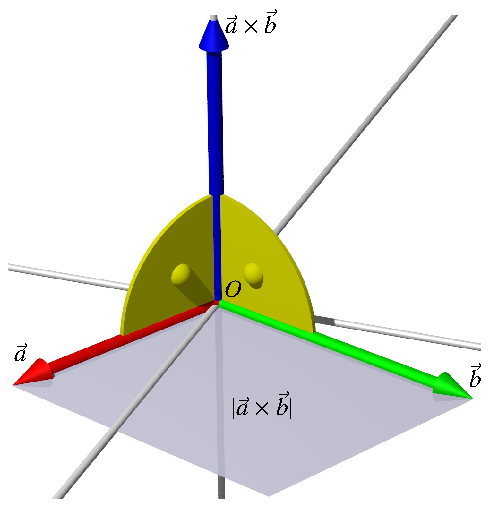
\includegraphics{5/images/vektorprodukt.pdf}
\caption{Das Vektorprodukt der Vektoren $\vec{a}$ und $\vec{b}$ ist ein Vektor
senkrecht auf $\vec{a}$ und $\vec{b}$ mit einer Länge, die dem 
Flächeninhalt des aufgespannten Parallelogramms entspricht und derart,
dass $\vec{a}$, $\vec{b}$ und $\vec{a}\times\vec{b}$ ein Rechtssystem
bilden.
\label{skript:vektorprodukt}}
\end{figure}
Das Vektorprodukt hat die folgenden Eigenschaften (siehe auch
Abbildung~\ref{skript:vektorprodukt}).
\begin{satz}
Sind $\vec a$ und $\vec b$ zwei dreidimensionale Vektoren, dann gilt
\begin{itemize}
\item $\vec a\times\vec b$ steht senkrecht auf $\vec a$ und $\vec b$.
\item $|\vec a\times\vec b|$ ist der Flächeninhalt des von
$\vec a$ und $\vec b$ aufgespannten Parallelogrammes im Raum
\item Ist $\alpha$ der Winkel zwischen $\vec a$ und $\vec b$, dann
ist
\[
|\vec a\times\vec b|=|\vec a|\,|\vec b|\sin \alpha.
\]
\end{itemize}
\end{satz}
\begin{proof}[Beweis]
Sei $\vec c$ ein Vektor in der von $\vec a$ und $\vec b$ aufgespannten
Ebene.
In diesem Fall degeneriert das Parallelepiped.
Es hat Volumen $0$,
also $V(\vec a,\vec b,\vec c)= 0$.
Da also
\[
V(\vec a,\vec b,\vec c)=(\vec a\times \vec b)\cdot \vec c=0,
\]
steht $\vec c$ senkrecht auf $\vec a\times\vec b$.
Da dies für jeden
Vektor $\vec c$ in der von $\vec a$ und $\vec b$ aufgespannten Ebene
gilt, steht $\vec a\times\vec b$ senkrecht auf dieser Ebene und insbesondere
auf $\vec a$ und $\vec b$.
Dies beweist die Aussage a).

Sei $\vec n$ der Normalenvektor mit Länge $1$ auf der von $\vec a$ und
$\vec b$ aufgespannten Ebene.
Das Volumen $V(\vec a,\vec b,\vec n)$ ist
dasjenige eines geraden Prismas mit dem von $\vec a$ und $\vec b$
aufgespannten Prisma mit Höhe $1$, also gleich gross wie der
Flächeninhalt des von $\vec a$ und $\vec b$ aufgespannten Parallelogramms.
Andererseits ist
\[
V(\vec a,\vec b,\vec n)=(\vec a\times\vec b)\cdot \vec n
\]
die Projektion des Vektors $\vec a\times\vec b$ auf $\vec n$.
Die beiden
Vektoren haben aber die gleiche Richtung, weil sie beide senkrecht stehen
auf der von $\vec a$ und $\vec b$ aufgespannten Ebene.
Also ist die Projektion
gerade die Länge des Vektors.
$|\vec a\times\vec b|$ ist also der Flächeninhalt des Parallelogramms.

Die Höhe des von $\vec a$ und $\vec b$ aufgespannten Parallelogramms
ist $|\vec b|\sin \alpha$, der Flächeninhalt also
$|\vec a\times\vec b|=|\vec a|\,|\vec b|\sin\alpha.$
\end{proof}

\begin{beispiel}
Man bestimme das Vektorprodukt von
\[
\vec a=\begin{pmatrix}1\\2\\3\end{pmatrix}
\quad\text{und}\quad
\vec b=\begin{pmatrix}8\\5\\13\end{pmatrix}.
\]

\smallskip
{\parindent 0pt Wir verwenden direkt die Definition}
\[
\vec a\times \vec b=
\begin{pmatrix}1\\2\\3\end{pmatrix}
\times
\begin{pmatrix}8\\5\\13\end{pmatrix}
=
\begin{pmatrix}
2\cdot 13-3\cdot 5\\
3\cdot 8-1\cdot 13\\
1\cdot 5-2\cdot 8
\end{pmatrix}
=
\begin{pmatrix}
11\\
11\\
-11
\end{pmatrix}.
\]
\end{beispiel}

\subsection{Normale}
Das Vektorprodukt erlaubt uns jetzt auf einfache Weise die Normale einer
Ebene zu finden.
Sei
\[
\vec r=\vec p+t\vec u+s\vec v
\]
die Parameterdarstellung einer Ebene, dann ist
\[
\vec n=\vec u\times\vec v
\]
eine Normale, also ist
\[
(\vec r-\vec p)\cdot (\vec u\times\vec v)=0
\]
die implizite Form der Ebenengleichung (Normalenform).

\begin{beispiel}
Man finde die Normale der Ebene mit der Gleichung (\ref{beispielebene}).

\smallskip
{\parindent 0pt Die Normale haben wir schon einmal mit Hilfe der Gleichungen
(\ref{gleichungen-fuer-normale}) berechnet, jetzt kann dies
mit Hilfe des Vektorproduktes vereinfacht werden:}
\begin{equation}
\vec n = \vec u\times \vec v=
\begin{pmatrix}2\\2\\-2\end{pmatrix}
\times
\begin{pmatrix}3\\-3\\-1\end{pmatrix}
=
\begin{pmatrix}
2\cdot(-1)-(-2)\cdot(-3)\\
(-2)\cdot 3-2\cdot (-1)\\
2\cdot(-3)-2\cdot 3
\end{pmatrix}
=
\begin{pmatrix}
-8\\
-4\\
-12
\end{pmatrix}
=-4\begin{pmatrix}2\\1\\3\end{pmatrix}.
\label{beispielvektorprodukt}
\end{equation}
$\vec{n}$ ist
also ein Vielfaches der mit den Gleichungen (\ref{gleichungen-fuer-normale})
gefundenen Normale.
Damit wird die Ebenengleichung
\begin{align*}
0=
\begin{pmatrix} -8\\ -4\\ -12 \end{pmatrix}\cdot
\left(
\begin{pmatrix}x\\y\\z\end{pmatrix}
-
\begin{pmatrix}1\\2\\1 \end{pmatrix}
\right)
&=
-8x-4y-12z+
28
\\
\Rightarrow
2x+y+3z&=7.
\end{align*}
\end{beispiel}

\subsection{Weitere Anwendungen}

\subsubsection{Zwischenwinkel}
Für den Zwischenwinkel zweier Vektoren gilt
\[
\sin\alpha=\frac{|\vec a\times\vec b|}{|\vec a|\cdot|\vec b|}.
\]
\begin{beispiel}
Berechne den Zwischenwinkel der Richtungsvektoren der Ebenengleichung
\ref{beispielebene}.

\smallskip

{\parindent 0pt Das Vektorprodukt der beiden Vektoren wurde
in (\ref{beispielvektorprodukt}) schon
berechnet.} Die Länge der Vektoren ist
\[
|\vec u|=\sqrt{4+4+4}=2\sqrt{3}
,
\quad
|\vec v|=\sqrt{9+9+1}=\sqrt{19}.
\]
Die Zwischenwinkelformel liefert jetzt
\begin{align*}
\sin\alpha&=\frac{|\vec u\times \vec v|}{|\vec u|\cdot |\vec v|}
=\frac{\sqrt{64+16+144}}{\sqrt{12\cdot 19}}
=\frac{\sqrt{224}}{\sqrt{228}}=0.98246\\
\alpha&=79.252^\circ.
\end{align*}
\end{beispiel}

\subsubsection{Die Schuhbändel-Formel für den Flächeninhalt eines Polygons}
\begin{figure}
\centering
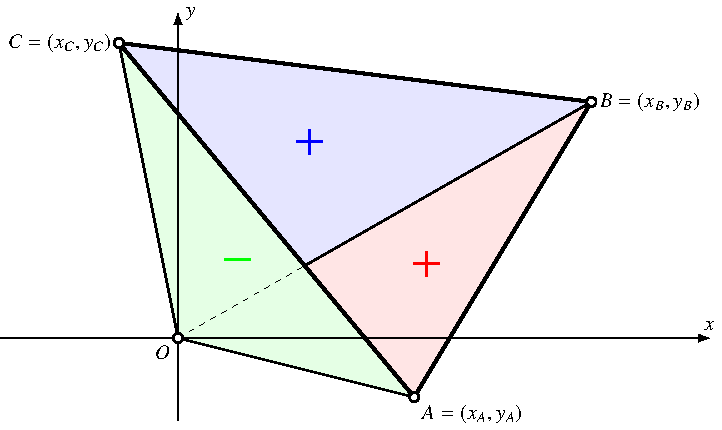
\includegraphics{5/images/schuhbaendel.pdf}
\caption{Schuhbändel-Formel zur Berechnung des Flächeninhalts eines
Polygons
\label{skript:orientierung:schuhbaendel}}
\end{figure}
Der orientierte Flächeninhalt eines Dreiecks $OAB$ in der Ebene wir durch
die halbe Determinante
\[
F(OAB)
=
\frac12\left|\,\begin{matrix} x_A&x_B\\y_A&y_B\end{matrix}\,\right|
=
\frac12\left|\,\begin{matrix} x_A&y_A\\x_B&y_B\end{matrix}\,\right|
\]
der Ortsvektoren $\vec{a}$ und $\vec{b}$ berechnet.
Kompliziertere Polygone können in Dreiecke zerlegt werden.
Der Flächeninhalt des Dreiecks $\triangle ABC$ in
Abbildung~\ref{skript:orientierung:schuhbaendel} zum 
Beispiel kann berechnet werden aus den orientierten Flächeninhalten
\begin{align*}
F(ABC)
&=
{\color{red}F(OAB)} + {\color{blue}F(OBC)} - {\color{green}F(OAC)}
\\
&=
{\color{red}F(OAB)} + {\color{blue}F(OBC)} + {\color{green}F(OCA)}
\\
&
=
\frac12 \left|\,\begin{matrix} x_A&x_B\\y_A&y_B\end{matrix}\,\right|
+
\frac12 \left|\,\begin{matrix} x_B&x_C\\y_B&y_C\end{matrix}\,\right|
+
\frac12 \left|\,\begin{matrix} x_C&x_A\\y_C&y_A\end{matrix}\,\right|
\\
&
=
\frac12 \left|\,\begin{matrix} x_A&y_A\\x_B&y_B\end{matrix}\,\right|
+
\frac12 \left|\,\begin{matrix} x_B&y_B\\x_C&y_C\end{matrix}\,\right|
+
\frac12 \left|\,\begin{matrix} x_C&y_C\\x_A&y_A\end{matrix}\,\right|.
\end{align*}
\begin{satz}{Schuhbändel-Formel}
Ein Polygon mit den Ecken $P_1,P_2,\dots,P_n$ hat den orientierten 
Flächeninhalt
\begin{equation}
F(P_1P_2\dots P_n) =
\frac12\left|\,\begin{matrix}x_1&y_1\\x_2&y_2\end{matrix}\,\right|
+
\frac12\left|\,\begin{matrix}x_2&y_2\\x_3&y_3\end{matrix}\,\right|
+\dots+
\frac12\left|\,\begin{matrix}x_n&y_n\\x_1&y_1\end{matrix}\,\right|
\label{skript:orientierung:schuhbaendel:satz}
\end{equation}
\end{satz}
\index{Schuhbändel-Formel}
Der Name Schuhbändel-Formel für
\eqref{skript:orientierung:schuhbaendel:satz}
kommt von der folgenden Erweiterung der Determinanten-Notation her:
\[
\left|\,
\begin{matrix}
x_1
\begin{picture}(0,0)
\color{red}
\drawline(1,-2)(8,-9)
\drawline(1,-9)(8,-2)
\end{picture}
&y_1\\
x_2
\begin{picture}(0,0)
\color{red}
\drawline(1,-2)(8,-9)
\drawline(1,-9)(8,-2)
\end{picture}
&y_2\\
x_3
\begin{picture}(0,0)
\color{red}
\drawline(1,-2)(8,-9)
\drawline(1,-9)(8,-2)
\end{picture}
&y_3\\
\vdots&\vdots\\
x_n
\begin{picture}(0,0)
\color{red}
\drawline(1,-2)(8,-9)
\drawline(1,-9)(8,-2)
\drawline(1,5.5)(8,12.5)
\drawline(1,12.5)(8,5.5)
\end{picture}
&y_n
\end{matrix}
\,\right|
=
\left|\,\begin{matrix}x_1
&y_1\\x_2&y_2\end{matrix}\,\right|
+
\left|\,\begin{matrix}x_2&y_2\\x_3&y_3\end{matrix}\,\right|
+
\dots
+
\left|\,\begin{matrix}x_n&y_n\\x_1&y_1\end{matrix}\,\right|.
\]
Der orientiert Flächeninhalt des Polygons kann damit als
\[
F(P_1P_2\dots P_n)
=
\frac12\left|\,
\begin{matrix}
x_1&y_1\\
x_2&y_2\\
x_3&y_3\\
\vdots&\vdots\\
x_n&y_n
\end{matrix}\,\right|
\]
geschriebenwerden.

\subsubsection{Abstand Punkt--Gerade}
\begin{figure}
\begin{center}
%\includegraphics{images/d-3}
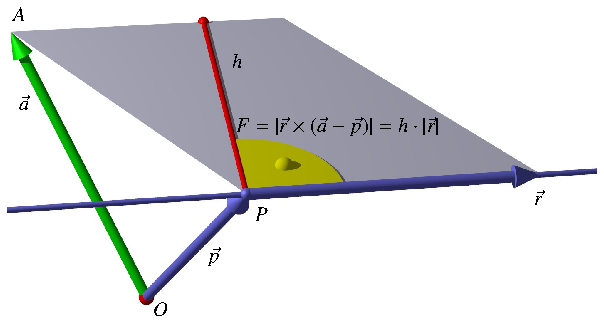
\includegraphics{5/images/abstand.pdf}
\end{center}
\caption{Abstand Punkt--Gerade mit dem Vektorprodukt\label{punkt-gerade}}
\end{figure}
Es ist der Abstand eines Punktes mit Ortsvektor $\vec a$ von der
Geraden durch den Punkt mit Ortsvektor $\vec p$ und Richtungsvektor $\vec r$,
also mit der Parameterdarstellung
\[
\vec q=\vec p+t\vec r
\]
zu bestimmen.
Der gesuchte Abstand $d$ ist die Höhe des Parallelogramms,
welches von $\vec a-\vec p$
und $\vec r$ aufgespannt wird, wobei $\vec r$ als Grundseite zu betrachten ist.
Der Flächeninhalt $A$ des Parallelogramms kann mit dem Vektorprodukt
berechnet werden:
\begin{align}
A
&=
|(\vec a-\vec p)\times\vec r|
\notag
\\
d
&=
\frac{|(\vec a-\vec p)\times\vec r|}{|\vec r|}.
\label{eqn:abstandpunktgerade}
\end{align}
\subsubsection{Abstand zweier windschiefer Geraden}
\begin{figure}
\begin{center}
%\includegraphics{images/d-4}
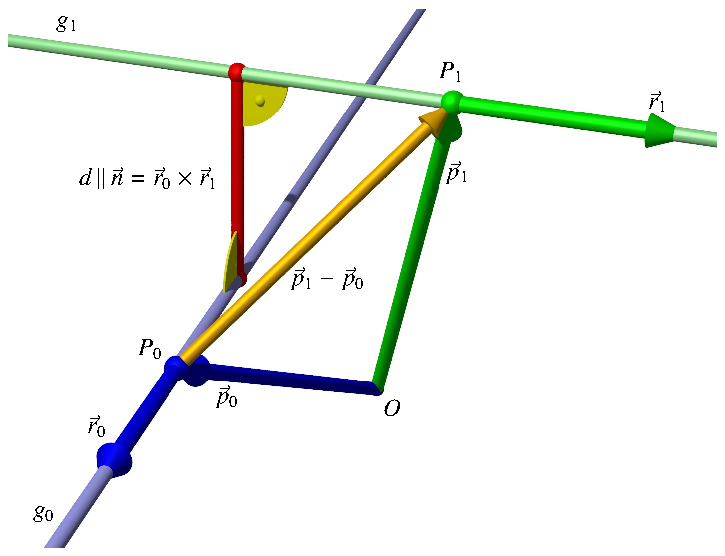
\includegraphics{5/images/windschief.pdf}
\end{center}
\caption{Abstand windschiefer Geraden: der minimale Abstand (rot) ist
parallel zur Normalen auf beide Geraden $g_0$ und $g_1$ also parallel
zum Vektorprodukt $\vec{r_0}\times\vec{r}_1$.
\label{windschief}}
\end{figure}
Zwei nicht parallele Geraden $g_0$ und $g_1$ im Raum,
die sich nicht schneiden, heissen
{\em windschief}.
\index{windschief}
Sie haben
einen kürzesten Abstand $d$, der auf beiden Geraden senkrecht steht.
Sind
\begin{align*}
g_0:
\vec p&=\vec p_0+t\vec r_0\\
g_1:
\vec p&=\vec p_1+t\vec r_1
\end{align*}
Parameterdarstellungen der Geraden, dann ist die Richtung des kürzesten
Abstandes die Richtung des Vektorproduktes $\vec n = \vec r_0\times\vec r_1$.
Ein Vektor zwischen zwei beliebigen Punkten auf den beiden Geraden,
zum Beispiel zwischen $P_0$ und $P_1$, also der Vektor $\vec p_1-\vec p_0$,
wird als Projektion auf die Richtung des kürzesten Abstandes immer die
Länge dieses kürzesten Abstandes haben.
Die Projektion kann mit dem
Skalarprodukt berechnet werden, der kürzeste Abstand $d$ ist
\begin{equation}
d
=
(\vec p_1-\vec p_0)
\cdot
\frac{\vec r_0\times\vec r_1}{|\vec r_0\times\vec r_1|}.
\label{eqn:windschieferabstand}
\end{equation}

